\section{Specifications}
\label{sec:specifications}
This chapter lays out the specification used to design the wavelength division modulation (WDM) system. See table \ref{table:specs1}, table \ref{table:specs2} and table \ref{table:specs3}.

\begin{table}[!ht]
	\centering
	\cite{noauthor_gofoton_nodate-1}
	\begin{tabular} {|l|c|}
		\hline
		\multicolumn{1}{|c|}{\textbf{Parameter}} & \textbf{Unit} \\ \hline\hline
		% Operating Wavelength & \unit{\nm} \\ \hline
		% Channel Spacing & \unit{\GHz} \\ \hline
		% Upgrade Port Wavelength Range (Option) & \unit{\nm} \\ \hline
		% Express Port Wavelength Range (Option) & \unit{\nm} \\ \hline
		% Pass Bandwidth & \unit{\nm} \\ \hline
		% Center Wavelength & \unit{\nm} \\ \hline
		% CWDM Port Insertion Loss & \unit{\dB} \\ \hline
		Passband WDL & \unit{\dB} \\ \hline
		% Express Port Wavelength (option) & \unit{\dB} \\ \hline
		% Upgrade Port Insertion Loss (option) & \unit{\dB} \\ \hline
		% Adjacent Channel Isolation & \unit{\dB} \\ \hline
		% Non-Adjacent Channel Isolation & \unit{\dB} \\ \hline
		% Upgrade Port Isolation & \\ \hline
		% Express port isolation & \\ \hline
		Polarization Dependent Loss & \unit{\dB} \\ \hline
		% Optical Return Loss & \unit{\dB} \\ \hline
		Directivity & \unit{\dB} \\ \hline
		% Optical Power Handling & \unit{\mW} \\ \hline
		Operating Temperature Range & \unit{\degreeCelsius} \\ \hline
		Storage Temperature Range & \unit{\degreeCelsius} \\ \hline
		Fiber Type & - \\ \hline
		Fiber Jacket & - \\ \hline
		Package Size & \unit{\mm} \\ \hline
		Number of Channels & - \\ \hline
		Accessibility & - \\ \hline
	\end{tabular}
	\caption{List of specifications GOFOTON CWDM}
	\label{table:specs1}
\end{table}

\begin{table}[!ht]
	\centering
	\cite{noauthor_4ch_nodate}
	\begin{tabular} {|l|c|}
		\hline
		\multicolumn{1}{|c|}{\textbf{Parameter}} & \textbf{Unit} \\ \hline\hline
		% Center Wavelength & \unit{\nm} \\ \hline
		% Channel Spacing & \unit{\nm} \\ \hline
		% Channel Passband & \unit{\nm} \\ \hline
		% Insertion Loss (Passband) & \unit{\dB} \\ \hline
		Technology & - \\ \hline
		Passband Ripple & \unit{\dB} \\ \hline
		Directivity & \unit{\dB} \\ \hline
		% Return Loss & \unit{\dB} \\ \hline
		PDL & \unit{\dB} \\ \hline
		PMD & \unit{\ps} \\ \hline
		% Power Handling & \unit{\mW} \\ \hline
		Operating Temperature & \unit{\degreeCelsius} \\ \hline
		Storage Temperature & \unit{\degreeCelsius} \\ \hline
		Connector Type & - \\ \hline
		Dimensions (H x W x D) & \unit{\mm} \\ \hline
	\end{tabular}
	\caption{List of specifications FS CWDM}
	\label{table:specs2}
\end{table}

\begin{table}[!ht]
	\centering
	\cite{noauthor_cisco_nodate-2}
	\begin{tabular} {|l|c|}
		\hline
		\multicolumn{1}{|c|}{\textbf{Parameter}} & \textbf{Unit} \\ \hline\hline
		% Channel center wavelength & \unit{\nm} \\ \hline
		% Channel spacing & \unit{\nm} \\ \hline
		% Maximum input optical power & \unit{\mW} \\ \hline
		% Insertion Loss & \unit{\dB} \\ \hline
		% Drop adjacent channel isolation & \unit{\dB} \\ \hline
		% Drop nonadjacent channel isolation & \unit{\dB} \\ \hline
		% Add adjacent channel isolation & \unit{\dB} \\ \hline
		% Add nonadjacent channel isolation & \unit{\dB} \\ \hline
		Add CrossTalk & \unit{\dB} \\ \hline
		% Return Loss & \unit{\dB} \\ \hline
		Monitor add/drop loss & \unit{\dB} \\ \hline
		Filter type & - \\ \hline
		Polarization dependent loss (PDL) & \unit{\dB} \\ \hline
		Polarization mode dispersion (PMD) & \unit{\ps} \\ \hline
		Insertion loss uniformity & \unit{\dB} \\ \hline
		Chromatic dispersion & \unit{\ps/\nm} \\ \hline
		Operating Temperature & \unit{\degreeCelsius} \\ \hline
		Storage Temperature & \unit{\degreeCelsius} \\ \hline
		Dimensions (H x W x D) & \unit{\mm} \\ \hline
		Connector Type & - \\ \hline
		% Channel Passband & \unit{\nm} \\ \hline
		% Technology & - \\ \hline
		% Passband Ripple & \unit{\dB} \\ \hline
		% Directivity & \unit{\dB} \\ \hline
		% Power Handling & \unit{\mW} \\ \hline
	\end{tabular}
	\caption{List of specifications Cisco CWDM}
	\label{table:specs3}
\end{table}

\begin{table}[!ht]
	\centering
	\begin{tabular}{|l|c|c|}
		\hline
		\multicolumn{1}{|c|}{\textbf{Parameter}} & \textbf{Value} & \textbf{Unit} \\ \hline
		Operating Wavelength & ITU-T G.694.2\cite{noauthor_g6942_2003} & \unit{\nm} \\ \hline
		Channel Center Wavelength & ITU-T G.694.2\cite{noauthor_g6942_2003} & \unit{\nm} \\ \hline
		Channel Spacing & 20\cite{noauthor_g6942_2003} & \unit{\nm} \\ \hline
		Channel Passband & \numrange[range-phrase=-]{\pm 6}{7}\cite{noauthor_g6942_2003} & \unit{\nm} \\ \hline
		Insertion Loss & TBD & \unit{\dB} \\ \hline
		Add Adjacent Channel Isolation & TBD & \unit{\dB} \\ \hline
		Add Non-Adjacent Channel Isolation & TBD & \unit{\dB} \\ \hline
		Drop Adjacent Channel Isolation & TBD & \unit{\dB} \\ \hline
		Drop Non-Adjacent Channel Isolation & TBD & \unit{\dB} \\ \hline
		Optical Power Handling & TBD & \unit{\mW} \\ \hline
		Return Loss & TBD & \unit{\dB} \\ \hline
	\end{tabular}
\end{table}

\subsection{Parameter definitions}

\begin{itemize}
	\item \textbf{Operating Wavelength}: Range of wavelengths used by the CWDM.
	\item \textbf{Channel Center Wavelength}: Set of channel wavelengths used by the CWDM.
	\item \textbf{Channel Spacing}: Wavelength difference between adjacent channels.
	\item \textbf{Channel Passband}: Maximum channel wavelength deviation.
	\item \textbf{Insertion Loss}: The amount of power lost in the device or at the interfaces.
	\item \textbf{Add}: Terminology for multiplexing\cite{noauthor_glossary_2015}.
	\item \textbf{Drop}: Terminology for de-multiplexing\cite{noauthor_glossary_2015}.
	\item \textbf{Adjacent Channel Isolation}: For any given channel, it is the difference between the maximum loss within the channels passband and the minimum loss within an adjacent channels passband\cite{noauthor_glossary_2015}.
	\item \textbf{Non-Adjacent Channel Isolation}: For any given channel, it is the difference between the maximum loss within the channels passband and the minimum loss within any other channels passband\cite{noauthor_glossary_2015}.
	\item \textbf{Optical Power Handling}: Maximum optical power at fiber inputs.
	\item \textbf{Return Loss}: The ratio of incident optical power vs reflected optical power for any given optical interface. Higher return loss leads to less signal loss and less power reflected to the source\cite{noauthor_glossary_2015}.
\end{itemize}
% \begin{itemize}
%  \item The inputs and outputs of the system are optical.
%  \item The signals will not be converted to the electrical domain at any stage (no O/E/O). 
%  \item Single mode fibre will be used.
%  \item 4 channels are used.
%  \item TX and RX signals use a common fiber.
%  \item The system can perform both MUX and DEMUX operations.
%  \item The channel wavelengths are spaced \qty{20}{\nm} apart.
% \end{itemize}

% The inputs and outputs of the system are all optical, as transponders fall outside the 
% scope of the system. By also keeping the signals in the optical domain, the mux and demux 
% operation has to be performed in the optical domain. Single mode fiber will be used, 
% meaning it is up to the user to make sure that each input is matched to the correct channel. 
% Single mode fiber was chosen such that modal dispersion doesn't have to be accounted for. 
% Lastly, individual channels will be spaced \qty{20}{\nm} apart, making it a CWDM system.

% From the above requirements a MUX/DEMUX system will be designed. An overiew of the of these 
% systems in a link is given in figure \ref{fig:link_overview}.

% \begin{figure}[ht]
%     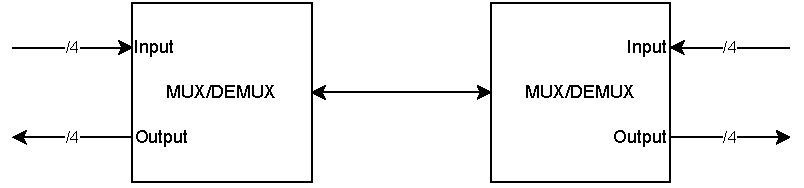
\includegraphics[width=\linewidth]{images/link_overview.pdf}
%     \caption{Overview of MUX/DEMUX link}
%     \label{fig:link_overview}
% \end{figure}